%  !TeX  root  =  user_guide.tex

\section{Stra�engraph Plugin}
\label{sec:roadgraph}
\index{Stra�engraph Erweiterung}
\index{K�rzester Weg}

% when the revision of a section has been finalized, 
% comment out the following line:
% \updatedisclaimer


Die \toolbtntwo{plugin}{Stra�engraph} Erweiterung ist ein C++ plugin, mit dem man 
die k�rzeste Verbindung zwischen zwei Punkten entlang eines Polyline Vektorlayers 
berechnen kann. Das Ergebnis kann als Shapefile gespeichert werden. 

\textbf{Hauptfunktionen}:

\begin{itemize}
\item Berechnung der Route, seiner L�nge und der Reisezeit
\item Optimierung durch L�nge oder Reisezeit
\item Export der Route als Vektorlayer
\item Anzeigen der Vektorrichtungen (diese Funktion ist langsam und wird meist 
nur zum Testen verwendet)
\end{itemize}

Als Netzwerk kann jeder Polyline Vektorlayer verwendet werden, der in einem von QGIS 
unterst�tzten Format gespeichert ist. Zwei Linien mit einem gemeinsamen Punkt werden 
dabei als verkn�pft angesehen. Wichtig ist, dass das Layer-KBS als Projekt-KBS gesetzt 
werden muss. Dies ist wichtig, da Neuberechnungen von Koordinaten ansonsten zu Fehlern 
f�hren k�nnen, selbst eine Fangtolleranz eintgestellt ist.

\textbf{In der Attributtabelle des Layera k�nnen folgende Spalten genutzt werden}:

\begin{itemize}
\item Geschwindigkeit als numerische Spalte;
\item Richtung in jedem Datentyp, der mit String kompatibel ist. Wenn eine Spalte 
benutzt wird, bezieht sie sich auf beide Richtungen, ansonsten wird unterschieden.
\end{itemize}

Wenn einige Zeilen keine Werte haben, werden die Defaultwerte verwendet. Sie k�nnen 
bei Bedarf ge�ndert werden, gemeinsam mit ein paar weiteren Einstellungsm�glichkeiten 
im Dialog \dialog{Stra�engraph-Einstellungen} im Menu \mainmenuopt{Vektor} \arrow 
\dropmenuopt{Stra�engraph}.

\minisec{Verwendung der Erweiterung}

Wenn Sie die Erweiterung laden, erscheint ein neues Fenster 'K�rzester Weg' unten 
links neben dem Kartenfenster. Legen Sie zu Beginn ein paar Einstellungen fest 
im Dialog \dialog{Stra�engraph-Einstellungen} im Menu \mainmenuopt{Vektor} \arrow 
\dropmenuopt{Stra�engraph}.

\begin{figure}[ht]
    \centering
    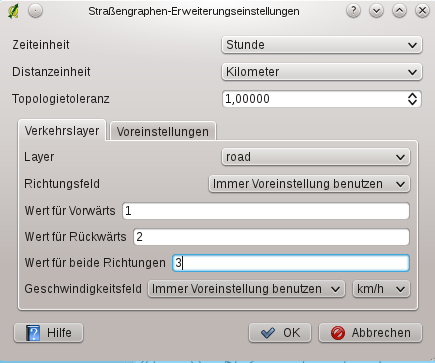
\includegraphics[clip=true, width=5cm]{roadgraph_settings}
    \caption{Einstellungen des Stra�engraph Plugin vornehmen \nixcaption}\label{fig:roadgraphsettings}
\end{figure}

W�hlen Sie nun einen Start- und einen Stop-Punkt im Vektorlayer auf dem Netzwerk und 
dr�cken Sie auf \button{Berechnen}.

\begin{figure}[ht]
    \centering
    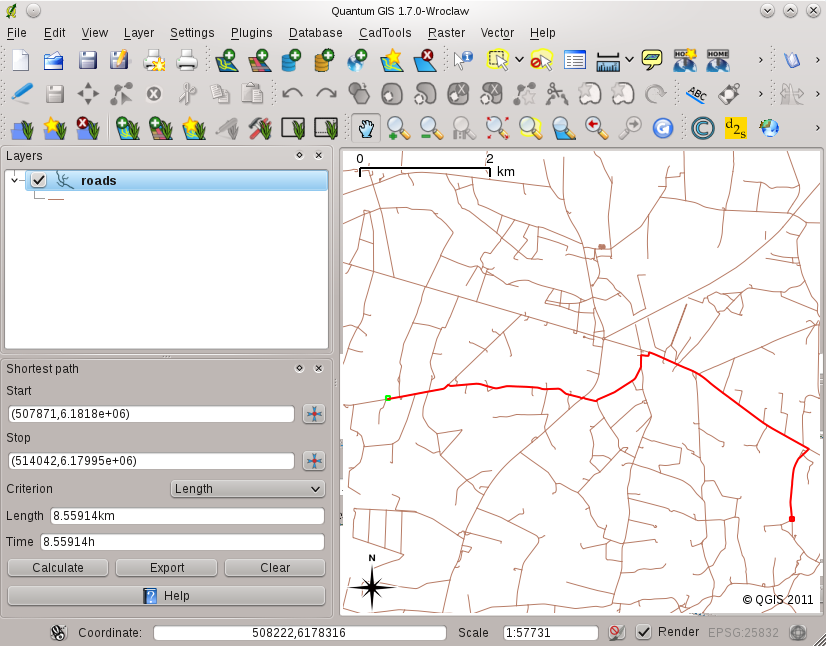
\includegraphics[clip=true, width=12cm]{roadgraph_sample}
    \caption{Stra�engraph Plugin \nixcaption}\label{fig:roadgraphsample}
\end{figure}

\FloatBarrier
